\section{Introduction to Field-level Inference}
\subsection{Definition and Motivations}

\subsubsection{Definition}

This definition is mostly taken from \cite{Leclercq_2025}. A field-level inference generally refers to methods and techniques used to infer 
physical fields alongside a set of parameters from observations, without relying on compressed data from the corresponding field. 
A field-level inference belongs to the class of inverse problems, whose objective is to infer the underlying causes of a set of observations by modeling the processes 
that generated them. In our case, we are interested in accessing the initial conditions of the underlying matter density field and velocity field. The goal is 
to extract the maximum amount of information regarding structure formation. 
By modeling the full field instead of relying on compressed summary 
statistics, one can incorporate more complex physical information. However, the inference becomes more sensitive to mismodeling and systematics, and could lead to more biased 
results if not accounted for properly.

\subsubsection{Motivations}

There are a number of motivating factors favoring the use of field-level inference rather than summary statistics when it comes to the study of structure formation. 
Unlike compressed statistics such as the matter power spectrum ($ \propto \left \langle \delta(\mathbf{k_1})  \delta(\mathbf{k_2})\right \rangle$), a field-level inference preserves all statistical 
information such as higher-order correlations \cite{Leclercq_2021}. The structures 
observed today are non-linear and non-Gaussian, meaning correlations of higher order such as the bispectrum ($ \propto \left \langle \delta(\mathbf{k_1})  \delta(\mathbf{k_2}) \delta(\mathbf{k_3})\right \rangle$) 
or trispectrum ($ \propto \left \langle \delta(\mathbf{k_1})  \delta(\mathbf{k_2}) \delta(\mathbf{k_3}) \delta(\mathbf{k_4})\right \rangle$) are non-zero and therefore contain additional 
information on cosmological parameters. Since the field-level inference aims at reconstructing the entire underlying field as well as its structures, these correlations will always 
be accounted for at all orders. Moreover it preserves phase information. The compressed statistics mainly calculate the amplitudes of the correlations that exist while missing out 
on the phase for which these amplitudes are possible. 
For example, the contribution of two overdense regions to the correlation function depends only on their separation and not on their absolute positions. 
Consequently, relocating the pair elsewhere in the Universe while preserving their separation would leave their contribution unchanged.

\noindent Another motivation for field-level inference is reducing the uncertainties that arise due to cosmic variance of the local-Universe. Traditional summary statistics assume ergodicity 
i.e. averaged measurements over a sufficiently large volume of the Universe approximate the averages over many hypothetical realizations, which becomes problematic in 
the local Universe due to the limited volume. With field-level inference, the goal is to reconstruct the specific realization that produces our observations, allowing us to 
properly adjust our model parameters to that realization (e.g. \cite{Porqueres_2021, Ramanah_2019}). 
The outcome of a field-level inference on observations of our Universe is what we call a Digital Twin, a cosmic variance-aligned numerical simulation of the dark matter 
density field that should, in theory, match the density field of our observable Universe. \\


\subsubsection{Performing a Field-level Inference}

Unlike the frequentist maximum likelihood approach adopted in the NaCl spectrophotometric framework, field-level inference is better suited using a Bayesian 
statistical framework. In the frequentist approach, parameters are treated as fixed unknowns and inferred by maximizing the likelihood 
$\mathcal{L}(d|\theta)$, where $d$ is the observed data and $\theta$ are a set of parameters, 
with uncertainties estimated from Fisher information matrix. This is well suited for NaCl as the number of parameters can be handled by a single personal computer. 
However, field-level inference involves a parameter space of order $N^3$ for an $N^3$ voxel 
grid. In our case $N$ can go from $64$ to $256$, giving us $10^5 - 10^7$ initial condition parameters alongside the model parameters (\cite{Jasche_2019,Mcalpine_2025}). 
Although maximum likelihood estimation can still be performed in such a high-dimensional space using gradient-based methods, 
efficiently exploring the full posterior distribution becomes considerably more challenging. 


The Bayesian framework addresses this by treating both data and parameters 
as random variables. The central equation comes from Bayes' theorem which states that the probability that an event $A$ occurs knowing an event $B$ has occurred is written as:
\begin{equation}
    \mathcal{P}(A|B) = \frac{\mathcal{P}(B|A) \cdot \mathcal{P}(A)}{\mathcal{P}(B)} = \frac{\mathcal{P}(A \cap  B)}{\mathcal{P}(B)}
\end{equation}
For a field-level inference, we are attempting to determine the initial conditions $\delta^{IC}$ and a set of model parameters $\theta$ given a set of observations $d$.
Ideally, we would like to determine the model of the Universe $M$ such as $\Lambda$CDM but this is not currently accessible and will be 
assumed as constant in our analysis (Section \ref{sec:BORG}).We nevertheless retain $M$ in the following expressions to illustrate 
the most general form of the posterior, but omit it in subsequent sections where the model is fixed. Thanks to Bayes' theorem, we get: 
\begin{equation}
    \mathcal{P}(\delta^{IC}, \theta, M | d) = \frac{\mathcal{P}(d | \delta^{IC}, \theta, M) \cdot \mathcal{P}(\delta^{IC}, \theta, M)}{\mathcal{P}(d)}
\end{equation}
The term $\mathcal{P}(d)$ is a constant with respect to the rest of the parameters so we will omit it for simplicity. 
Using the chain rule decomposition $\mathcal{P}(A, B|C) = \mathcal{P}(A|C) \cdot \mathcal{P}(B|A, C)  $, we can rewrite the full posterior as:
\begin{equation}
    \mathcal{P}(\delta^{IC}, \theta, M | d) = \mathcal{P}(M | d) \cdot \mathcal{P}(\delta^{IC}, \theta | d, M)
\end{equation}
\begin{equation}
    \mathcal{P}(\delta^{IC}, \theta, M | d) = \mathcal{P}(M | d) \cdot \mathcal{P}(\theta | d, M) \cdot \mathcal{P}(\delta^{IC} | d, M, \theta)
    \label{eqn:bayesian_borg}
\end{equation}
We can see three distinct terms:
\begin{itemize}
    \item The term $\mathcal{P}(M | d)$ describes which cosmological model fits the data best ($\Lambda$CDM or $w$CDM, GR or modified gravity, etc...). 
    \item The term $\mathcal{P}(\theta | d, M)$ estimates the model parameters given the data and a cosmological model ($\Omega_m$, $\sigma_8$, bias model parameters, etc...).
    \item The term $\mathcal{P}(\delta^{IC} | d, M, \theta)$ estimates the initial conditions for a specific realization of the Universe, given the data, a model and its parameters.
\end{itemize}
The posterior naturally distinguishes between regions of 
the density field that are well constrained by the data and those that are not, where the posterior defaults to a prior specified beforehand. The nuisance parameters 
can be marginalized, integrated over their full posterior distribution, which correctly propagates all their uncertainty into the parameters of interest, unlike 
in the frequentist approach which explores only a restricted region of the full parameter space. \\

The inherent high dimensionality of these analyses requires advanced statistical techniques. First, a differentiable forward model is generally employed to describe the 
evolution of the initial matter field and enable the use of gradient-based sampling methods. Second, the inference algorithm must be computationally efficient to make 
the exploration of the high-dimensional parameter space tractable. 

\subsection{Field-level Inference Pipeline}

\subsubsection{The BORG Framework}

This PhD work uses the \textit{Bayesian Origin Reconstruction from Galaxies} (BORG) (\cite{Jens_2013, Jasche_2019}), a field-level forward model framework designed to 
reconstruct the initial conditions of the Universe given a set of observations. 


The BORG framework is illustrated in Figure \ref{fig:BORG_schematic} and is composed of three main ingredients. First, 
the forward model generates Gaussian initial conditions on a grid of $N^3$ voxels, models the nonlinear 
evolution with a gravity model and connects the nonlinear matter density field to the 
observable of interest. Second, the data likelihood has an explicit functional form that depends on 
the observable of interest, for instance for application to galaxy surveys, we may use a Poisson 
likelihood for galaxy counts. The third component is the parameter sampler that needs to be 
efficient enough in order to sample the very high dimensional parameter space. Moreover, BORG 
employs a modular parameter sampler design that allows any additional parameters introduced 
by a model component to be included through a Gibbs sampling scheme. 
The BORG algorithm will be described in more detail in Section \ref{sec:BORG}. 
Applications of BORG to simulated and real data will be discussed in Section \ref{sec:applications_fli}. 

\begin{figure}[ht]
    \centering
    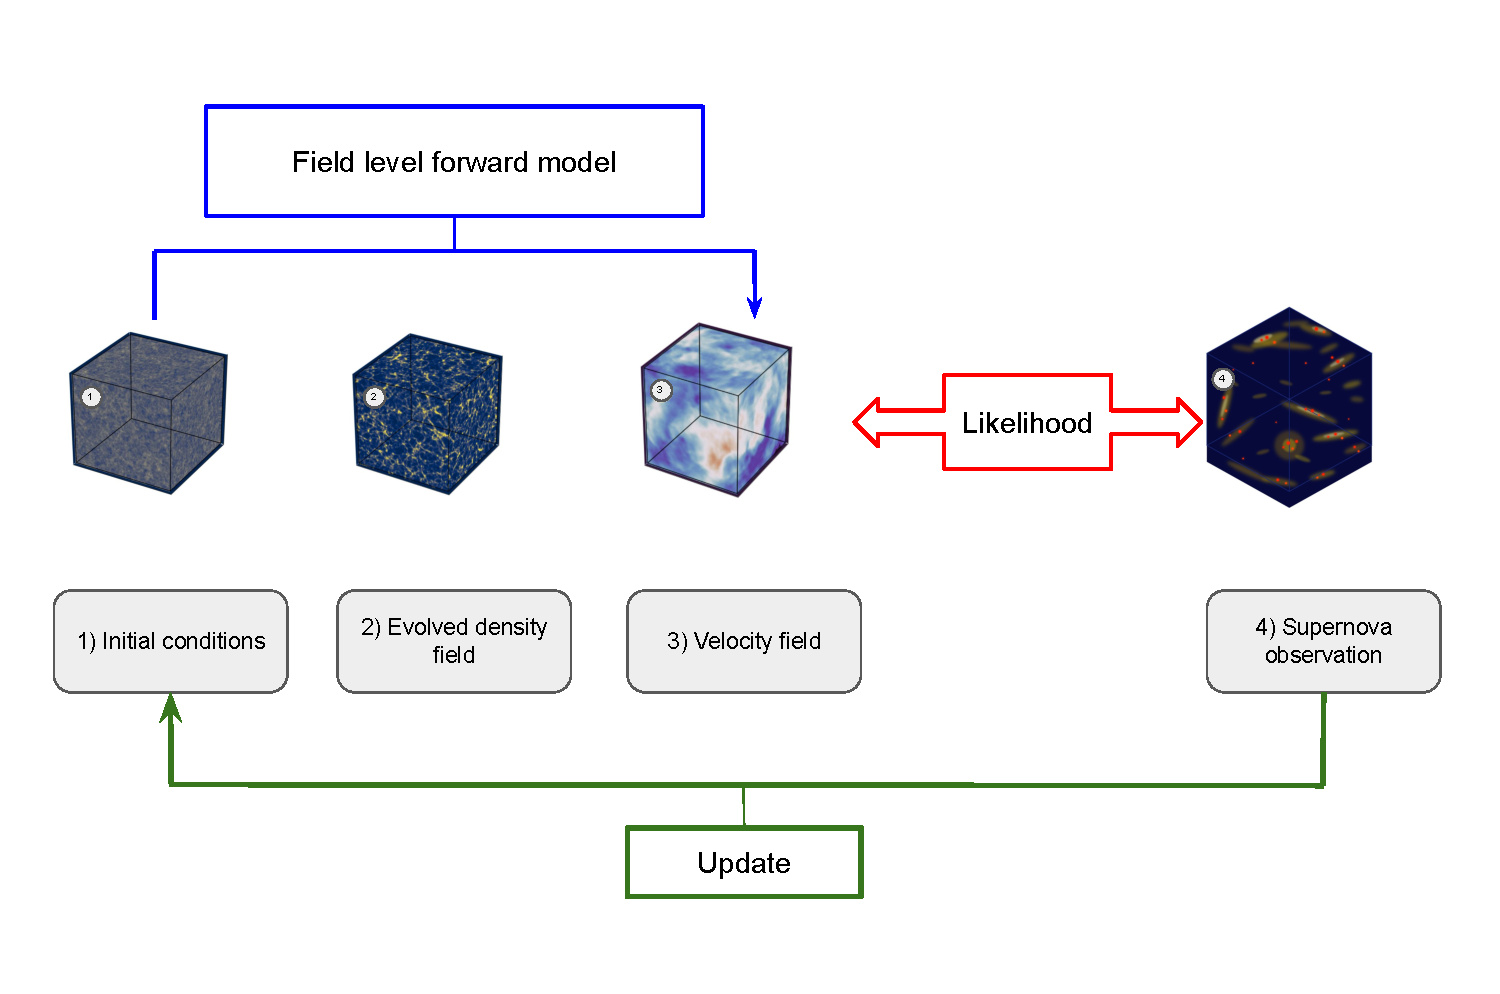
\includegraphics[width=1.0\textwidth]{MainLayout/BORG_chapter/figures/BORG_sn_schematic.pdf}
    \caption{Schematic summarizing what BORG intends to do when faced with Type Ia supernova data. First we start with a set of initial conditions. The initial conditions 
    then evolve using a gravity solver to obtain the density field today. Observational effects are applied to match the observations, such as selection effects and 
    survey footprint. Finally we evaluate a likelihood. The goal is to adjust the initial conditions and the model parameters to maximize the likelihood. Adapted from \url{https://indico.ijclab.in2p3.fr/event/8881/contributions/28072/attachments/20421/28316/COPHY_Lavaux.pdf}.}
    \label{fig:BORG_schematic}
\end{figure}

\subsubsection{Other Approaches}

As described in the previous section, BORG is arguably the most advanced end-to-end field-level inference 
pipeline. Other approaches have been developed, in this section we will describe two of them. 

The first one is 
the FlowPM model (\cite{Modi_2020}), a differentiable cosmological N-body simulator using the Particle Mesh (PM) gravity solver (more details in Section \ref{sec:gravity_model}) 
designed to run on GPU for accelerated results using a neural network framework. It was shown to be able to reconstruct 
cosmological fields when implemented in a forward model Bayesian framework. This model was tested only on simulations. 

The second model was developed by \cite{Simon_2025} based on the JaxPM\footnote{\url{https://github.com/DifferentiableUniverseInitiative/JaxPM}} 
gravity solver, an N-body simulator using PM coded in Python-Jax and can run on GPU. The model was tested using different samplers and they highlight the importance of carefully preconditioning 
latent variables in the model in order to achieve unbiased results on simulations. It also highlighted the differences between the samplers and the different algorithms that can be used to 
sample the likelihood. 

More recently, works by \cite{Bayer_2026} demonstrated the capabilities of running a field-level inference when trying to reconstruct the BAO signal 
in comparison to traditional methods where a hybrid Effective Field Theory approach was applied instead of a PM gravity solver. The results have shown an improvement in the 
BAO signal reconstruction using field-level inference in comparison to standard methods. \\


\subsection{Applications of Field-level Inference in Cosmology} \label{sec:applications_fli}

\subsubsection{Galaxy Clustering}

Examples of direct applications on real galaxy clustering data are the Manticore products obtained with the BORG forward model (\cite{Jens_2013, Jasche_2019}). Manticore-Local (\cite{Mcalpine_2025}) is a set of reconstructed dark matter simulations to 
match the observations in the 2M++ galaxy catalogue (\cite{Lavaux_2011}) with galaxies up to a redshift of $z \lesssim 0.1$. Manticore-Deep (\cite{Mcalpine_2026}) extends the work done on Manticore-Local 
by applying the algorithm on five galaxy catalogues 2M++, 6dFGS, 2dFGRS, SDSS, and BOSS (\cite{Lavaux_2011,Jones_2009_6dFGS,Colless_2003_2dFGRS,
York_2000_SDSS,Dawson_2013_BOSS}) reaching a redshift of $z \lesssim 0.7$, the largest Digital Twin that exists to date at a resolution of $\sim 4 \, h^{-1}.\text{Mpc}$. 
This gives us access to more than just cosmological parameters but a better understanding of the local 
structures in the Universe by being able to observe them one by one like the Virgo cluster or the Great Attractor. 
It also allows us to access hard-to-observe properties such as the velocity field, formation histories and tidal fields. 
It can also be used to further the study of void catalogues 
which are sensitive probes of the dark matter fields as it was done in \cite{Malandrino_2026}. \\


There is also the work of \cite{Nguyen_2024} on the study of galaxy clustering at the field level on simulations. 
The paper focuses primarily on the constraints obtained on the $\sigma_8$ 
parameter. Two methods were used to constrain the parameter on two N-body dark matter mocks' halos. 
The first method uses a differentiable forward model that incorporates a non linear gravity 
solver LEFTfield (\cite{Schmidt_2021}) that combines Effective Field Theory and Lagrangian Perturbation Theory (see Section \ref{sec:gravity_model}) and 
evolves the initial conditions 
to match the simulated halos. The use of the fully evolved field gives direct access to the cosmological parameters. The second method extracts the cosmological 
parameters from 
the power spectrum and bispectrum of the mocks ($P+B$ method). The results obtained show improvements on the $\sigma_8$ constraints with the field-level inference 
with a factor of 1.9 to 5.2 
based on the limiting modes included in the analysis ($k_{\text{max}} = 0.10 h \text{Mpc}^{-1}$ and $k_{\text{max}} = 0.12 h \text{Mpc}^{-1}$ respectively)
and the mock used. Figure \ref{fig:nguyen} shows the constraints obtained from methods on one of the mocks. \\ 

\begin{figure}[ht]
    \centering
    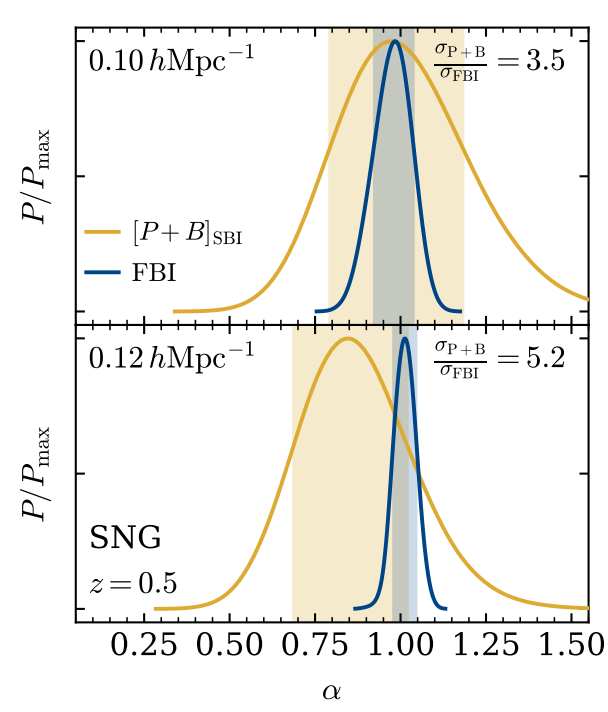
\includegraphics[width=0.6\textwidth]{MainLayout/BORG_chapter/figures/nguyen.png}
    \caption{Posterior distribution of the reconstructed value of $\sigma_8 /\sigma_{8, \text{true}} $. In blue are the results from the field-level inference and 
    in yellow are the results from the $P+B$ method. The top Figure is for a limiting mode of $k_{\text{max}} = 0.10 h \text{Mpc}^{-1}$ and the bottom for 
    $k_{\text{max}} = 0.12 h \text{Mpc}^{-1}$. Taken from \cite{Nguyen_2024}.}
    \label{fig:nguyen}
\end{figure}


\subsubsection{Weak Lensing}

The following study highlights the constraining power of field-level inference. It was done by \cite{Porqueres_2023, Porqueres_2021} on simulated weak lensing catalogues. 
The study was conducted using the 
BORG framework. The developed hierarchical forward model included astrophysical systematics of intrinsic alignment and baryon feedback in addition to the gravity 
solver. The resulting model has been called BORG-WL. The model was tested on self-consistent simulations and was used to constrain both the matter content $\Omega_m$ and 
$\sigma_8$. This was then compared to the traditional summary statistics by inferring the parameters using the angular power spectrum. They obtain the following results in 
Figure \ref{fig:porqueres}. The results show much tighter constraints on both parameters as well as being able to break the degeneracy between them. However, 
there is no uncertainty associated with photometric redshift or shape measurement that were accounted for in this work. \\

\begin{figure}[ht]
    \centering
    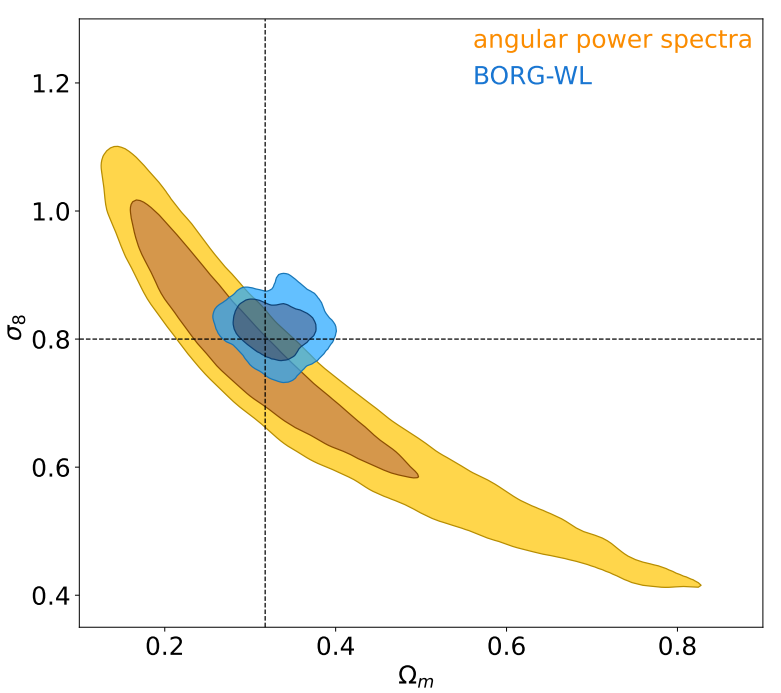
\includegraphics[width=0.6\textwidth]{MainLayout/BORG_chapter/figures/porqueres.png}
    \caption{Comparison of $\Omega_m$-$\sigma_8$ constraints from BORG-WL (blue) and the angular power spectrum (yellow) for self-consistent mocks. Taken from \cite{Porqueres_2023}.}
    \label{fig:porqueres}
\end{figure}


\subsubsection{Primordial non-Gaussianities}

Primordial non-Gaussianities (PNGs) are small deviations from the Gaussian statistics of the primordial density perturbations. 
Their detection would provide valuable insight into the physics of inflation, as different inflationary scenarios predict distinct non-Gaussian signatures (\cite{Chen_2010}). 
An application of field-level inference to this problem was first presented by \cite{Andrews_2023}, where the BORG framework was extended to 
jointly infer the initial conditions and the local primordial non-Gaussianity parameter $f_{\text{NL}}$. 
Applied to SDSS-III/BOSS-like mock galaxy catalogues, the method achieved a factor of $\sim2.5$ improvement over the observational constraints available at the time.

More recently, \cite{Andrews_2026} extended this framework to realistic halo catalogues generated from the Quijote N-body simulations (\cite{Villaescusa_2020}). 
Compared to a joint power spectrum and bispectrum analysis, the field-level approach achieved a factor of $\sim1.3$ improvement in the 
uncertainty on $f_{\text{NL}}$. The inference was also tested on multiple gravity solvers to assess the impact of resolving small-scales on the measurement of $f_{\text{NL}}$.


\subsubsection{Peculiar Velocities}


We present several studies that assess the performance of field-level inference for reconstructing the cosmic velocity field. 
A widely used approach for reconstructing the local velocity field is the linear reconstruction method of \cite{Carrick_2015}, 
which uses the luminosity-weighted galaxy density field from the 2M++ survey \cite{Lavaux_2011}. 
While such linear reconstructions provide an effective description of the large-scale velocity field, they do not fully capture the non-linear gravitational 
evolution of structure on smaller scales. 
Recent comparisons of local Universe reconstructions have demonstrated the importance of 
accounting for these non-linearities when reconstructing the velocity field \cite{Stiskalek_2025_b}. 


We first consider the work of \cite{Boruah_2020}, which reconstructed the large-scale velocity field from the 2M++ galaxy survey \cite{Lavaux_2011} using the linear 
reconstruction method of \cite{Carrick_2015}. The reconstructed velocity field was subsequently compared with independent peculiar velocity measurements 
from Type Ia supernovae and Tully-Fisher catalogues, allowing for a measurement of $f\sigma_8$. 
However, subsequent work has shown that the inferred $f\sigma_8$ is sensitive to calibration effects and to the cosmic variance associated 
with the finite survey volume (\cite{Hollinger_2024}). 
The field-level approach adopted in this work instead incorporates the peculiar velocity tracers directly into the inference of the underlying density and velocity fields. 
This provides a unified framework in which the information from the tracers, together with the measurement uncertainties and the 
uncertainties associated with the reconstructed fields, is propagated jointly through the inference. 
Rather than using the peculiar velocity measurements only to assess an independently reconstructed velocity field, they directly contribute to constraining the field itself. \\


The second study, by \cite{Prideaux_Ghee_2022}, extended the BORG framework to reconstruct the initial matter density and velocity fields directly from peculiar velocity tracers 
using Lagrangian Perturbation Theory (LPT). 
The method was validated using mock catalogues extracted from \texttt{GADGET2} N-body simulations (\cite{Springel_2005}). 
Their results demonstrated that accurate velocity field reconstructions can be achieved by incorporating peculiar velocity tracers directly into a Bayesian field-level 
inference, even when using an approximate gravitational forward model. 
In particular, the use of Lagrangian perturbation theory allowed the reconstruction to extend into the mildly non-linear regime, as illustrated in Figure \ref{fig:james_vel}.
This motivates the use of non-linear 
gravity solvers when attempting to reconstruct the velocity field from 
peculiar velocity tracers.  
However, the implementation remains a proof of concept. 
The authors identify the use of more accurate non-linear gravity and velocity models as an important direction for future work. 
Furthermore, their validation is performed using mock tracers, with some 
simplifying assumptions regarding the observed distances. 
Applications to real data would therefore require accounting for the fact 
that the observed distance modulus provides an estimate of the true distance, 
and propagating the associated uncertainty through the field-level inference. \\

\begin{figure}[ht]
    \centering
    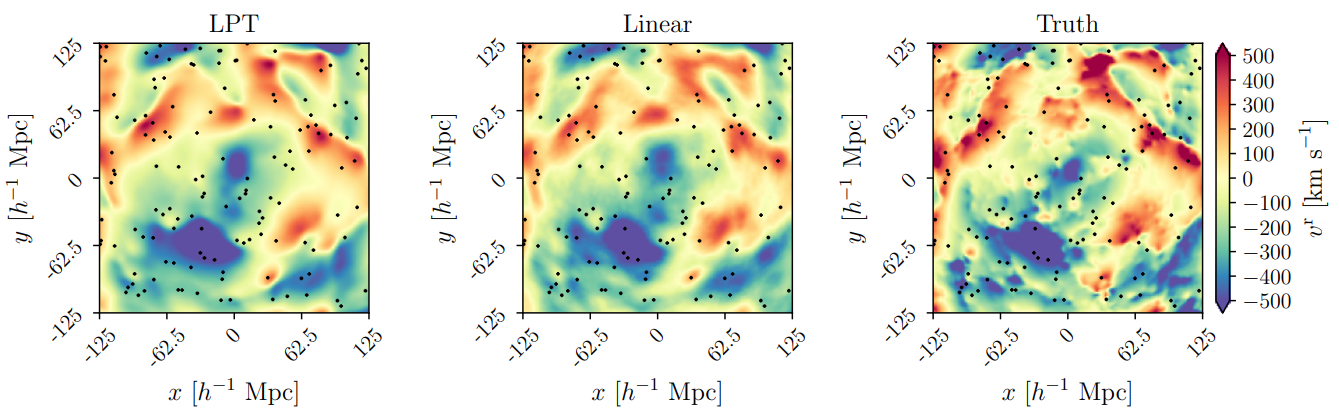
\includegraphics[width=0.9\textwidth]{MainLayout/BORG_chapter/figures/james_vel.png}
    \caption{Comparison of reconstructed velocity fields from \cite{Prideaux_Ghee_2022}. \textit{Left:} reconstruction using Lagrangian Perturbation Theory (LPT), 
    which captures mildly non-linear gravitational evolution. \textit{Center:} reconstruction using linear perturbation theory. \textit{Right:} reference velocity 
    field from the \texttt{GADGET2} N-body simulation.}
    \label{fig:james_vel}
\end{figure}



Lastly, we present the study conducted by \cite{Stiskalek_2025_b} on the reconstruction of velocity fields. The paper compares different methods in reconstructing the velocity field 
from a reconstruction of the local Universe to peculiar velocity catalogues from direct distance tracers.  
Each reconstruction can be used to infer the velocity field. We will list the different local Universe reconstruction methods 
in Table \ref{tab:velocity_olympics} and show the results from the different methods in Figure \ref{fig:olympics_dens}, which highlights how accounting for non-linearities in the 
gravity model translates onto the small scales of the density fields. 
It is important to note that amongst those methods, 
the CSiBORG1 and CSiBORG2 reconstructions are field-level inferences with BORG.  

\begin{table}[ht]
    \centering
    \caption{Different local Universe reconstruction methods.}
    \label{tab:velocity_olympics}
    \begin{tabularx}{\textwidth}{|l|c|X|c|}
    \hline
    Model & Alias & Description & Resolution \\
    \hline
    \cite{Carrick_2015}
    & C15
    & Linear inverse modelling using a luminosity-weighted galaxy density field. Used the 2M++ galaxy catalogue \cite{Lavaux_2011}. & $4\,h^{-1}\,\text{Mpc}$. \\
    \hline
    \cite{Lilow_2024}
    & L24
    & Machine-learning inverse method trained on Quijote simulations. Used the 2MRS galaxy catalogue \cite{Huchra_2012}. & $3.1\,h^{-1}\,\text{Mpc}$. \\
    \hline
    \cite{Jasche_2019}
    & CSiBORG1
    & BORG forward model. Used the 2M++ galaxy catalogue. & $2.6\,h^{-1}\,\text{Mpc}$. \\
    \hline
    \cite{Stopyra_2023}
    & CSiBORG2
    & BORG forward model with an improved gravity solver. Used the 2M++ galaxy catalogue. & $2.6\,h^{-1}\,\text{Mpc}$. \\
    \hline
    \cite{Sorce_2018, Sorce_2020}
    & S18
    & Constrained realization using a Wiener filter, which combines the peculiar velocity measurements with prior statistical information, and the reverse Zel'dovich approximation. Used CosmicFlows-2 peculiar velocities \cite{Tully_2013}. & $1.9\,h^{-1}\,\text{Mpc}$. \\
    \hline
    \cite{Courtois_2023}
    & C23
    & HMC sampling of the density field at $z=0$ constrained by peculiar velocities. Used CosmicFlows-4 peculiar velocities \cite{Tully_2023}. & $3.9\,h^{-1}\,\text{Mpc}$. \\
    \hline
    \end{tabularx}
    \end{table}


\begin{figure}[ht]
    \centering
    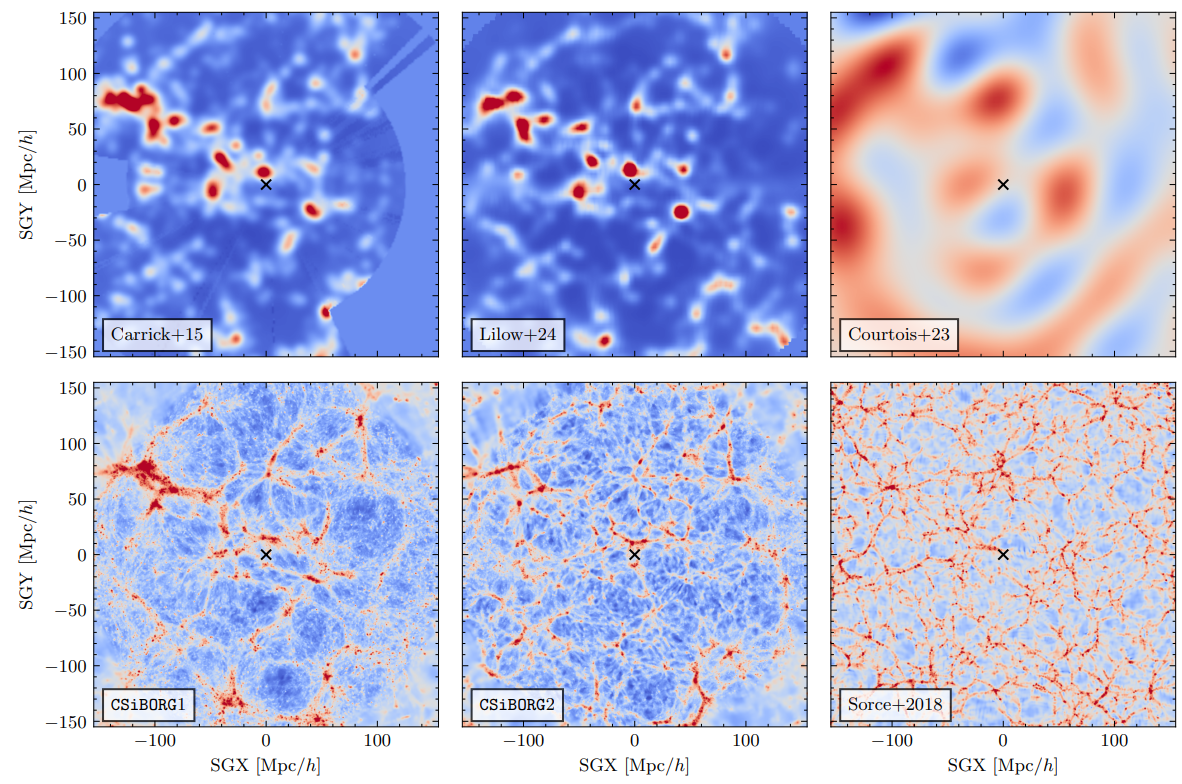
\includegraphics[width=0.9\textwidth]{MainLayout/BORG_chapter/figures/olympics_dens.png}
    \caption{Slice of the reconstructed matter field from each method used and described in Table \ref{tab:velocity_olympics}. The slices were chosen to look at the same portion 
    of the sky.}
    \label{fig:olympics_dens}
\end{figure}

The velocity fields are then compared to peculiar velocities from Tully-Fisher and one from Type Ia supernova catalogues. 
There are multiple metrics used to assess how accurate the velocity field reconstructions are, mainly relying on computing the evidence $\mathcal{Z}$ , i.e the probability of observing the 
peculiar velocities given a model. This is presented in Figure \ref{fig:olympics_rank} where we can see that the BORG reconstruction outperforms the other models. This highlights the importance 
of accounting for non-linearities when it comes to assessing velocity fields. 
The better performance of the BORG reconstructions 
therefore demonstrates the importance of modeling non-linear gravitational 
evolution when predicting the velocity field on the scales probed by peculiar 
velocity tracers. This motivates moving beyond traditional linear velocity 
reconstructions and incorporating non-linear structure formation directly 
within the inference. \\

In this work, we adopt such a field-level approach using the BORG framework, 
where the peculiar velocity tracers directly constrain the underlying density 
and velocity fields through a non-linear forward model. In the next section we will describe the core of the BORG framework. 

\begin{figure}[ht]
    \centering
    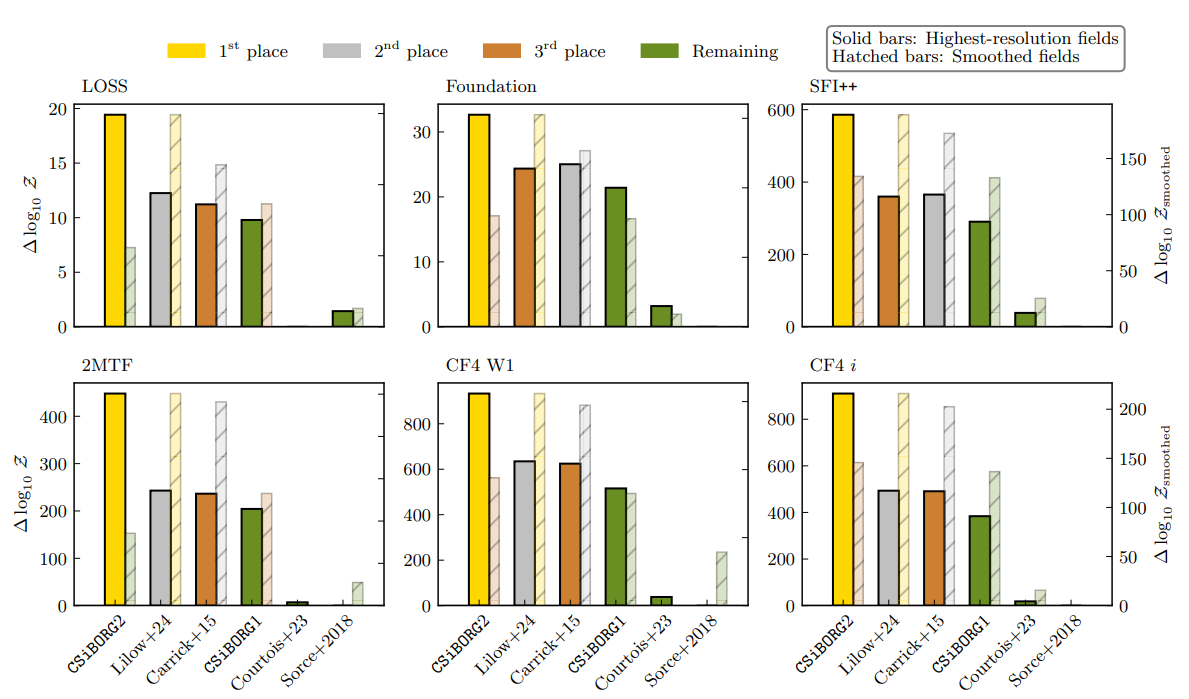
\includegraphics[width=0.9\textwidth]{MainLayout/BORG_chapter/figures/olympics_rank.png}
    \caption{Logarithmic evidence for each method highlighting in gold the most accurate reconstruction then silver, bronze and green in that order. The evidence was calculated 
    for six peculiar velocity catalogues. The LOSS and Foundation catalogues are supernova catalogues while the remaining ones are Tully-Fisher catalogues. Taken from \cite{Stiskalek_2025_b}.}
    \label{fig:olympics_rank}
\end{figure}
